\documentclass[10pt]{beamer}

\usecolortheme{dove}
\definecolor{mycyan}{rgb}{0.2157, 0.7059, 0.9608}
\setbeamercolor{alerted text}{fg=mycyan}
\setbeamertemplate{bibliography item}{\insertbiblabel}
\setbeamertemplate{caption}[numbered]
\hypersetup{colorlinks,linkcolor=,urlcolor=mycyan}
\usepackage{animate,xcolor,colortbl,nicefrac}
\usepackage[italian]{babel}
\usepackage{listings}
\lstset{upquote=false}
\usepackage[]{framed}
\begin{document}


\begin{frame}
  \title{Metodi di Krylov}
  \subtitle{Metodi per la soluzione numerica di sistemi di equazioni lineari non simmetriche applicabili in un sottospazio di Krylov.}
  \date{29/04/2020}
  \author[Principal]{Fabio Archenti \and Fabio Camagni \and Andrea Favero \and  \\Lorenzo Fiamingo \and Stefano Gallivanone \and Nazariy Nashkolnyy}
  \maketitle
\end{frame}

\begin{frame}
    \frametitle{Bibliografia}
    
  \begin{thebibliography}{99}\small
    \bibitem{quarteroni2012calcolo}
    Quarteroni, Saleri, and Gervasio.
    \newblock {\em Calcolo Scientifico: Esercizi e problemi risolti con MATLAB e  Octave}.
    \newblock UNITEXT. Springer Milan, 2012.

    \bibitem{trefethen-bau}
    Trefethen, and Bau.
    \newblock {\em Numerical Linear Algebra}.
    \newblock SIAM, 1997.
    
   
   \bibitem{dac95}
   Telichevesky, Kundert, and White.
   \newblock {\em Efficient Steady-State Analysis based on Matrix-Free Krylov-Subspace Methods}.
   \newblock {\em Scientific report}, June 1995.

   \end{thebibliography}

%Una volta inserito un documento in bibliografia, 
%può essere citato così:~\cite{quarteroni2012calcolo}
  
\end{frame}  

\begin{frame}
  \frametitle{Sommario}
  %Questo comando inserisce una lista delle sezioni in
  %cui è divisa la presentazione. Perché una sezione appaia 
  %nel sommario deve contenere almeno una pagina.
  \tableofcontents
\end{frame}

\section{Introduzione}\label{sec:sec1}

%\begin{frame} \frametitle{Motivazioni}
%\begin{itemize}
%    \item Utilizziamo allora i metodi iterativi (subspaziali di Krylov), il cui scopo è minimizzare la norma del residuo partendo da una soluzione approssimata.
%\end{itemize}
%\end{frame}

\begin{frame} \frametitle{Introduzione}
\begin{itemize}
    \item I metodi di Krylov risolvono sistemi lineari A$\mathbf{x}=\mathbf{b}$, dove:
    \begin{itemize}
    \item $A\in\mathbb{C}^{n\times n}$ è una matrice quadrata
    \item $\mathbf{x}\in\mathbb{C}^{n}$ è il vettore delle incognite
    \item $\mathbf{b}\in\mathbb{C}^{n}$ è il vettore dei termini noti
    \end{itemize}
    \item Ad ogni passo dell'iterazione viene calcolata una soluzione approssimata $\mathbf{x}_k$ appartenente al sottospazio di Krylov:
    \item Si definisce \alert{sottospazio di Krylov} il sottospazio generato:
    $$
    \mathcal{K}_\mathrm{n}(A,\mathbf{b})=span\{\mathbf{b},A\mathbf{b},A^2\mathbf{b},\dots,A^{n-1}\mathbf{b}\}\text{, } n\geq1
    $$.
    %\begin{itemize}
   % \item A causa dell'applicazione del metodo delle potenze è probabile che i vettori diventino linearmente dipendenti: sono quindi necessari metodi di ortogonalizzazione.
    %\end{itemize}
    
\end{itemize}
\end{frame} 

\begin{frame} \frametitle{Introduzione (II)}
\begin{itemize}
    \item $\mathbf{x}_0$ è la \alert{guess} iniziale al passo $0$.
    \item Definiamo la \alert{soluzione} del sistema cercata $$\mathbf{x}^*=A^{-1}\mathbf{b}$$
    \item Definiamo il \alert{residuo} del sistema al passo $k$
    $$\mathbf{r}_k =\mathbf{b}-A\mathbf{x}_k$$
    \item Definiamo l'\alert{errore} del sistema al passo $k$
    $$\mathbf{e}_k =\mathbf{x}_k-\mathbf{x}^*$$
    Possiamo notare come $\mathbf{r}_k=-A^{-1}\mathbf{e}_k$.
\end{itemize}
\end{frame} 




\begin{frame} \frametitle{Metodi di discesa}
\begin{itemize}
    \item Data A matrice simmetrica e definita positiva, possiamo definire la funzione (detta \alert{forma quadratica}) $\phi:\mathbb{R}^n \to \mathbb{R}$ $$\phi(\mathbf{x})=\frac{1}{2}\mathbf{x}^TA\mathbf{x}-\mathbf{x}^T\mathbf{b}$$
    \item Questa funzione (se le ipotesi su A sono verificate) è una funzione convessa e ammette un unico punto $\mathbf{x}^{\ast}$ di \alert{minimo assoluto}.
    
\end{itemize}
\begin{figure}
    \centering
    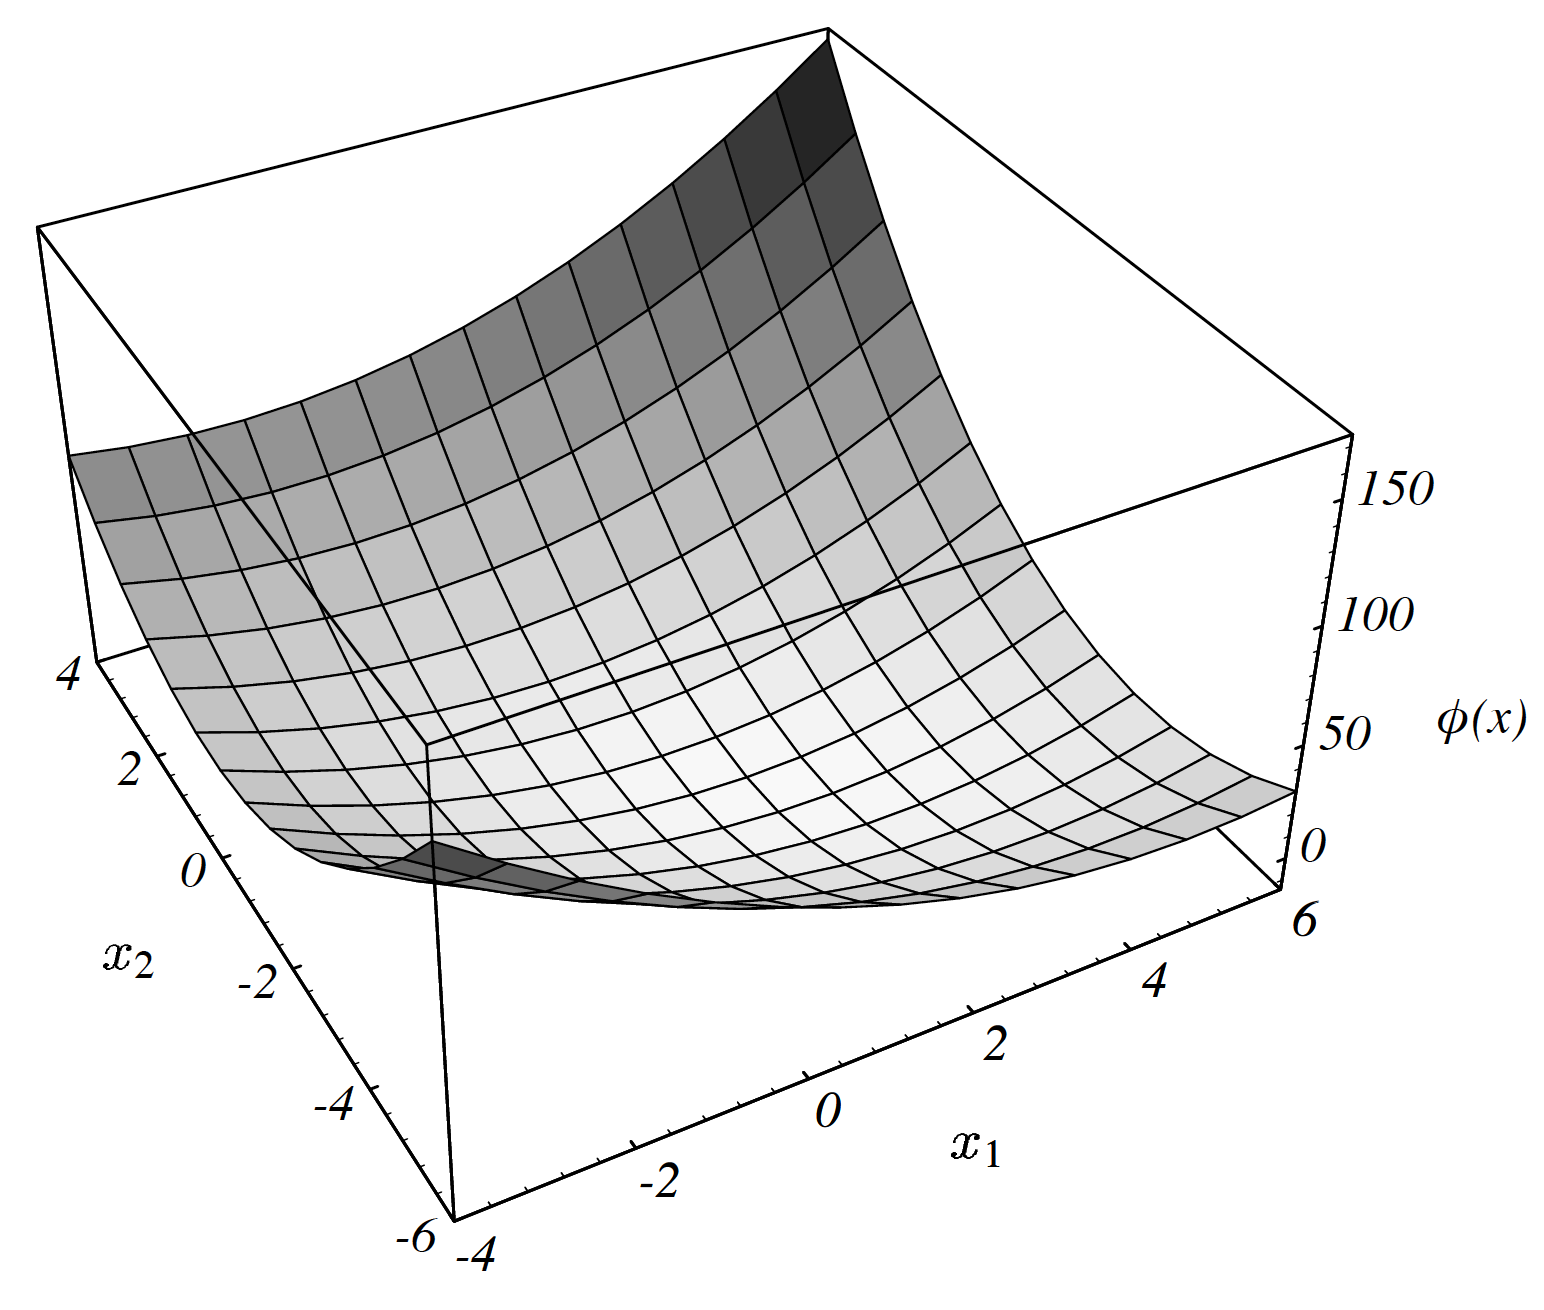
\includegraphics[width=.25\linewidth]{cg_quad.png}
    \caption{Forma quadratica per una matrice definita positiva}
    \label{fig:quad}
\end{figure}
\end{frame}

\begin{frame} \frametitle{Metodi di discesa (II)}
 \begin{itemize}
 \item Calcolo del \alert{gradiente} di $\phi(\mathbf{x})$: $\nabla\phi(\mathbf{x}) = A\mathbf{x}-\mathbf{b}$ (con $\nabla(\mathbf{b}^T\mathbf{x}) = \mathbf{b}$ e $\nabla(\mathbf{x}^T A \mathbf{x}) = 2A\mathbf{x}$).
 
 \item Nel punto $\mathbf{x}^{\ast}$ il gradiente si annulla:  $\nabla \phi(\mathbf{x}^{\ast})=A\mathbf{x}^{\ast}-\mathbf{b}=\mathbf{0}$.
 Risolvere il problema di minimo su $\phi(\mathbf{x})$ (trovando $\mathbf{x}^{\ast}$) equivale quindi a risolvere il sistema A$\mathbf{x}=\mathbf{b}$.

 \item Assegnato un $\mathbf{x}_0\in \mathbb{R}^n$, si procede per ogni $\mathit{k}$ fino a convergenza:
    \begin{enumerate}
        \item determinando una direzione di discesa $\mathbf{d_k} \in \mathbb{R}^n$
        \item determinando un passo $\alpha_k\in \mathbb{R}$
        \item ponendo $\mathbf{x}_{k+1}=\mathbf{x}_{k}+\alpha_k\mathbf{d}_{k}$
    \end{enumerate}
    
 %\item Condizioni per direzione di discesa: %per una funzione $\phi$ è un vettore d tale che: (in un punto x generico) 
  %   \begin{enumerate}
   %     \item $\mathbf{d}^T\nabla\phi(\mathbf{x}) < 0$, se $\nabla\phi(\mathbf{x})  != 0$
    %    \item $\mathbf{d} = \mathbf{0}$, se $\nabla\phi(\mathbf{x}) = 0$
%    \end{enumerate}

    \item L'approccio sarà lo stesso per il metodo del Gradiente e per il metodo del Gradiente Coniugato, ma sceglieremo direzioni di discesa $\mathbf{d}_{k}$ diverse per ogni metodo.

\end{itemize}
\end{frame}

\begin{frame}{Metodo del Gradiente}

\begin{itemize}
    \item Per il metodo del Gradiente la direzione $\mathbf{d}_k$ è il residuo $\mathbf{r}_k =\mathbf{b}-A\mathbf{x}_k$.
    
    \item $\nabla\phi(\mathbf{x}) = A\mathbf{x} - \mathbf{b}$: $\mathbf{d}_k = \mathbf{r}_k = - \nabla\phi(\mathbf{x})$.
    
    \item Si può dimostrare che il passo di discesa ottimale è $\alpha_k=\frac{\mathbf{d}_k^T \mathbf{r}_k}{\mathbf{d}_k^T A \mathbf{d}_k}$.
    
    \item Si aggiorna la soluzione: $\mathbf{x}_{k+1}=\mathbf{x}_{k}+\alpha_k\mathbf{d}_{k}$.
    
    \item E infine si aggiorna il residuo: $\mathbf{r}_{k+1}=\mathbf{r}_{k}-\alpha_kA\mathbf{d}_{k}$.
\end{itemize}
\begin{figure}
    \centering
    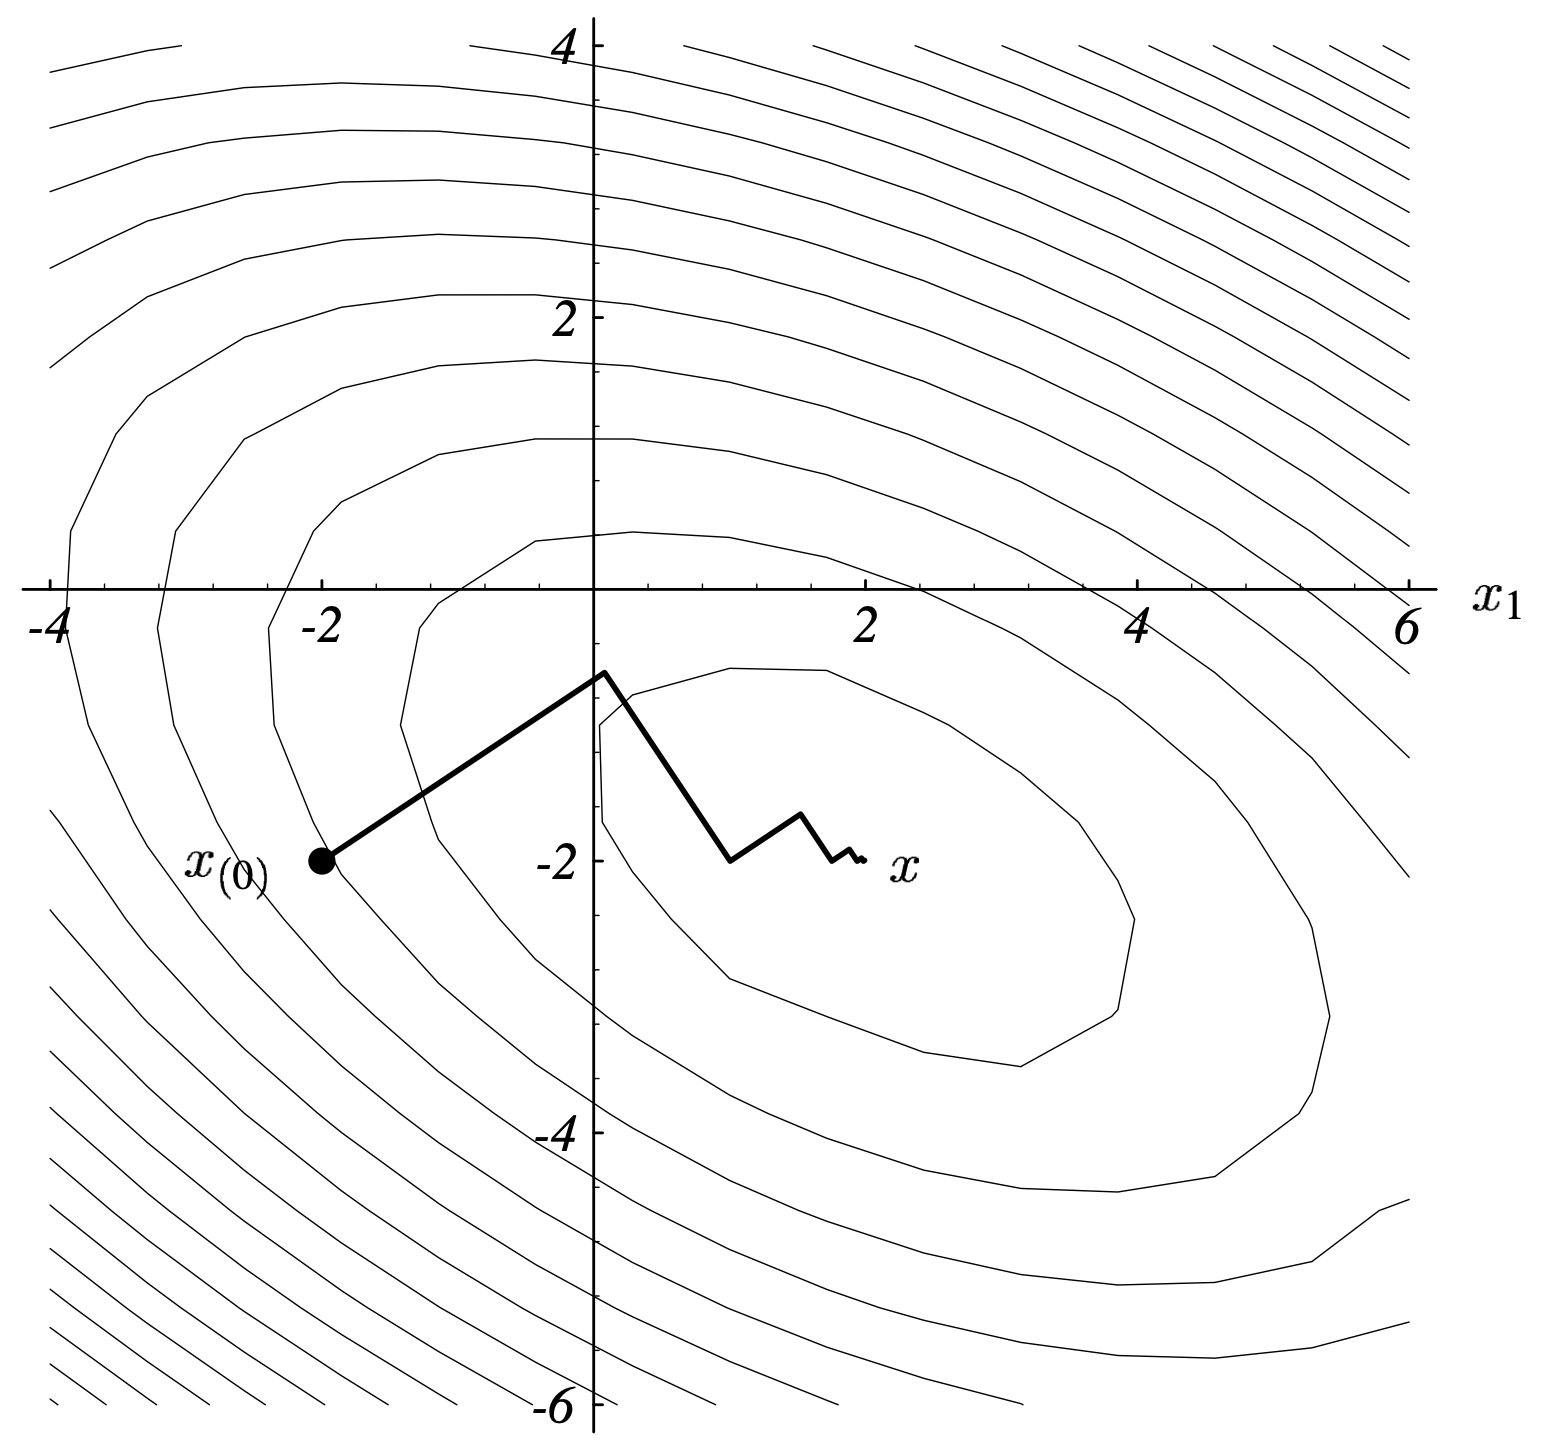
\includegraphics[width=.4\linewidth]{cg_grad.png}
    \caption{Iterazioni del metodo del gradiente}
    \end{figure}    
\end{frame}

\section{Metodo del Gradiente Coniugato}\label{sec:sec2}
\begin{frame} \frametitle{Metodo del Gradiente Coniugato - Passo di discesa}
\begin{itemize}

\item Il \alert{passo di discesa} più conveniente (che minimizza $\phi(\mathbf{x_{k+1}})$) è
$$\alpha_k=\frac{\mathbf{d}_k^T \mathbf{r}_k}{\mathbf{d}_k^T A \mathbf{d}_k}$$ .

\item Dimostrazione:
\begin{itemize}
    \item Sostituendo la soluzione al passo $k+1$ $\mathbf{x}_{k+1}=\mathbf{x}_{k}+\alpha_k\mathbf{d}_{k}$ nella forma quadratica
    $$\phi(\mathbf{x_{k+1}})=\phi(\mathbf{\mathbf{x}_{k}+\alpha_k\mathbf{d}_{k}})=
    \frac{1}{2}\left(\mathbf{d}_k^TA\mathbf{d}_k\right)\alpha_k^2
    -\mathbf{d}_k^T\underbrace{\left(\mathbf{b}-A\mathbf{x}_k\right)}_{=\mathbf{r}_k}\alpha_k
    +\frac{1}{2}\mathbf{x}_k^TA\mathbf{x}_k
    -\mathbf{x}_k^T\mathbf{b}
    $$
    
    \item Derivando e imponendo la condizione di stazionarietà
    $$
    \frac{d\phi}{d\alpha_k}(\mathbf{\mathbf{x}_{k}+\alpha_k\mathbf{d}_{k}})=
    \left(\mathbf{d}_k^TA\mathbf{d}_k\right)\alpha_k
    -\mathbf{d}_k^T\mathbf{r}_k=0
    $$
    \item Ricaviamo $\alpha_k$ ottenendo la formula cercata.
    
    \end{itemize}

\end{itemize}
\end{frame}

\begin{frame} \frametitle{Calcolo del residuo}
\begin{itemize}

\item Calcoliamo il \alert{residuo} $\mathbf{r}_k =\mathbf{b}-A\mathbf{x}_k$:
$$\mathbf{r}_{k+1}=\mathbf{r}_k-\alpha_kA\mathbf{d}_{k}$$ .

\item Dimostrazione:
\begin{itemize}
    \item $\mathbf{r}_{k+1}=-A\mathbf{e}_{k+1}$
    \item $\mathbf{r}_{k+1}=-A\left(\mathbf{e}_k+\alpha_k\mathbf{d}_k \right)$
    \item $\mathbf{r}_{k+1}=\mathbf{r}_k-\alpha_kA\mathbf{d}_{k}$
    
    \end{itemize}

\item Questa formula, in caso di matrici di grandi dimensioni, potrebbe essere soggetta ad errori di troncamento. Una buona soluzione potrebbe essere l'utilizzare $\mathbf{r}_k =\mathbf{b}-A\mathbf{x}_k$ dopo alcune iterazioni.
\end{itemize}
\end{frame}

\begin{frame} \frametitle{Direzione di discesa}
\begin{itemize}
%\item Affinchè $\{\mathbf{d}_k\}$ siano $A$-ortogonali e ottenute a partire da $\{\mathbf{r}_k\}$  $\mathbf{d}_{j}^TA\mathbf{d}_{k+1}=\mathbf{r}_{k+1}^T\mathbf{d}_j=\mathbf{0}$ per $j=0,\dots,k$
\item Utilizziamo l'\alert{ortogonalizzazione di Gram-Schmidt} per ottenere direzioni $\{\mathbf{d}_k\}$ $A$-ortogonali a partire dai residui $\{\mathbf{r}_k\}$
\begin{itemize}
\item $\mathbf{d}_0=\mathbf{r}_0$
\item $\mathbf{d}_{k+1}=\mathbf{r}_{k+1}+\sum_{h=0}^k\beta_{kh}\mathbf{d}_h$
\end{itemize}
\item Dato che $A\mathcal{K}_k$ è incluso in $\mathcal{K}_{k+1}$, il fatto che $\mathbf{r}_{k+1}$ sia ortogonale a $\mathcal{K}_{k+1}$ implica che $\mathbf{r}_{k+1}$ sia $A$-ortogonale a $A\mathcal{K}_k$, e quindi a tutte le precedenti direzioni di discesa $\mathbf{d}$, esclusa $\mathbf{d}_k$. 
\item Di conseguenza \alert{non sarà necessario memorizzare le vecchie direzioni} per assicurare la $A$-ortogonalità delle nuove.
\item La \alert{direzione di discesa} diviene
$$
\mathbf{d}_{k+1}=\mathbf{r}_{k+1}+\beta_{k+1}\mathbf{d}_k
$$
dove
$$
\beta_{k+1}=\frac{\mathbf{r}_{k+1}^T\mathbf{r}_{k+1}}{\mathbf{r}_{k}^T\mathbf{r}_{k}}
$$
\end{itemize}
\end{frame}


%\begin{frame} \frametitle{Scelta della direzione di discesa}
%\begin{itemize}
    
%    \item Scegliamo ad ogni passo una direzione $A$-ortogonale rispetto a tutte le direzioni precedenti, cioè tale che $(A\mathbf{d}_{j})^T\mathbf{d}_{k+1}=\mathbf{0}$ e $(\mathbf{r}_{k+1})^T\mathbf{d}_j=\mathbf{0}$ con $j=0,\dots,k$.
    
 %   \item All'inizio $\mathbf{d}_0=\mathbf{r}_0$, poi $(\mathbf{d}_{k+1})=\mathbf{r}_{k+1}-\beta_k\mathbf{d}_k$ per $k=0,\dots,n-1$, con $\beta_k=\frac{(A\mathbf{d}_{k})^T\mathbf{r}_{k+1}}{(A\mathbf{d}_{k})^T\mathbf{d}_{k}}$ (scelta ottimale).
    
 %   \item In questo modo le $\mathbf{d}_k$ sono linearmente indipendenti e la soluzione $\mathbf{x}_{k+1}$ è ottimale rispetto a tutte le direzioni di discesa (ovvero $\mathbf{r}_{k+1}$ è ortogonale a $\mathbf{d}_k$): è garantito che $\mathbf{x}_n=\mathbf{x}^{\ast}$.
%\end{itemize}
%\end{frame}

\begin{frame} \frametitle{Passo di discesa (II)}
\begin{figure}
    \centering
    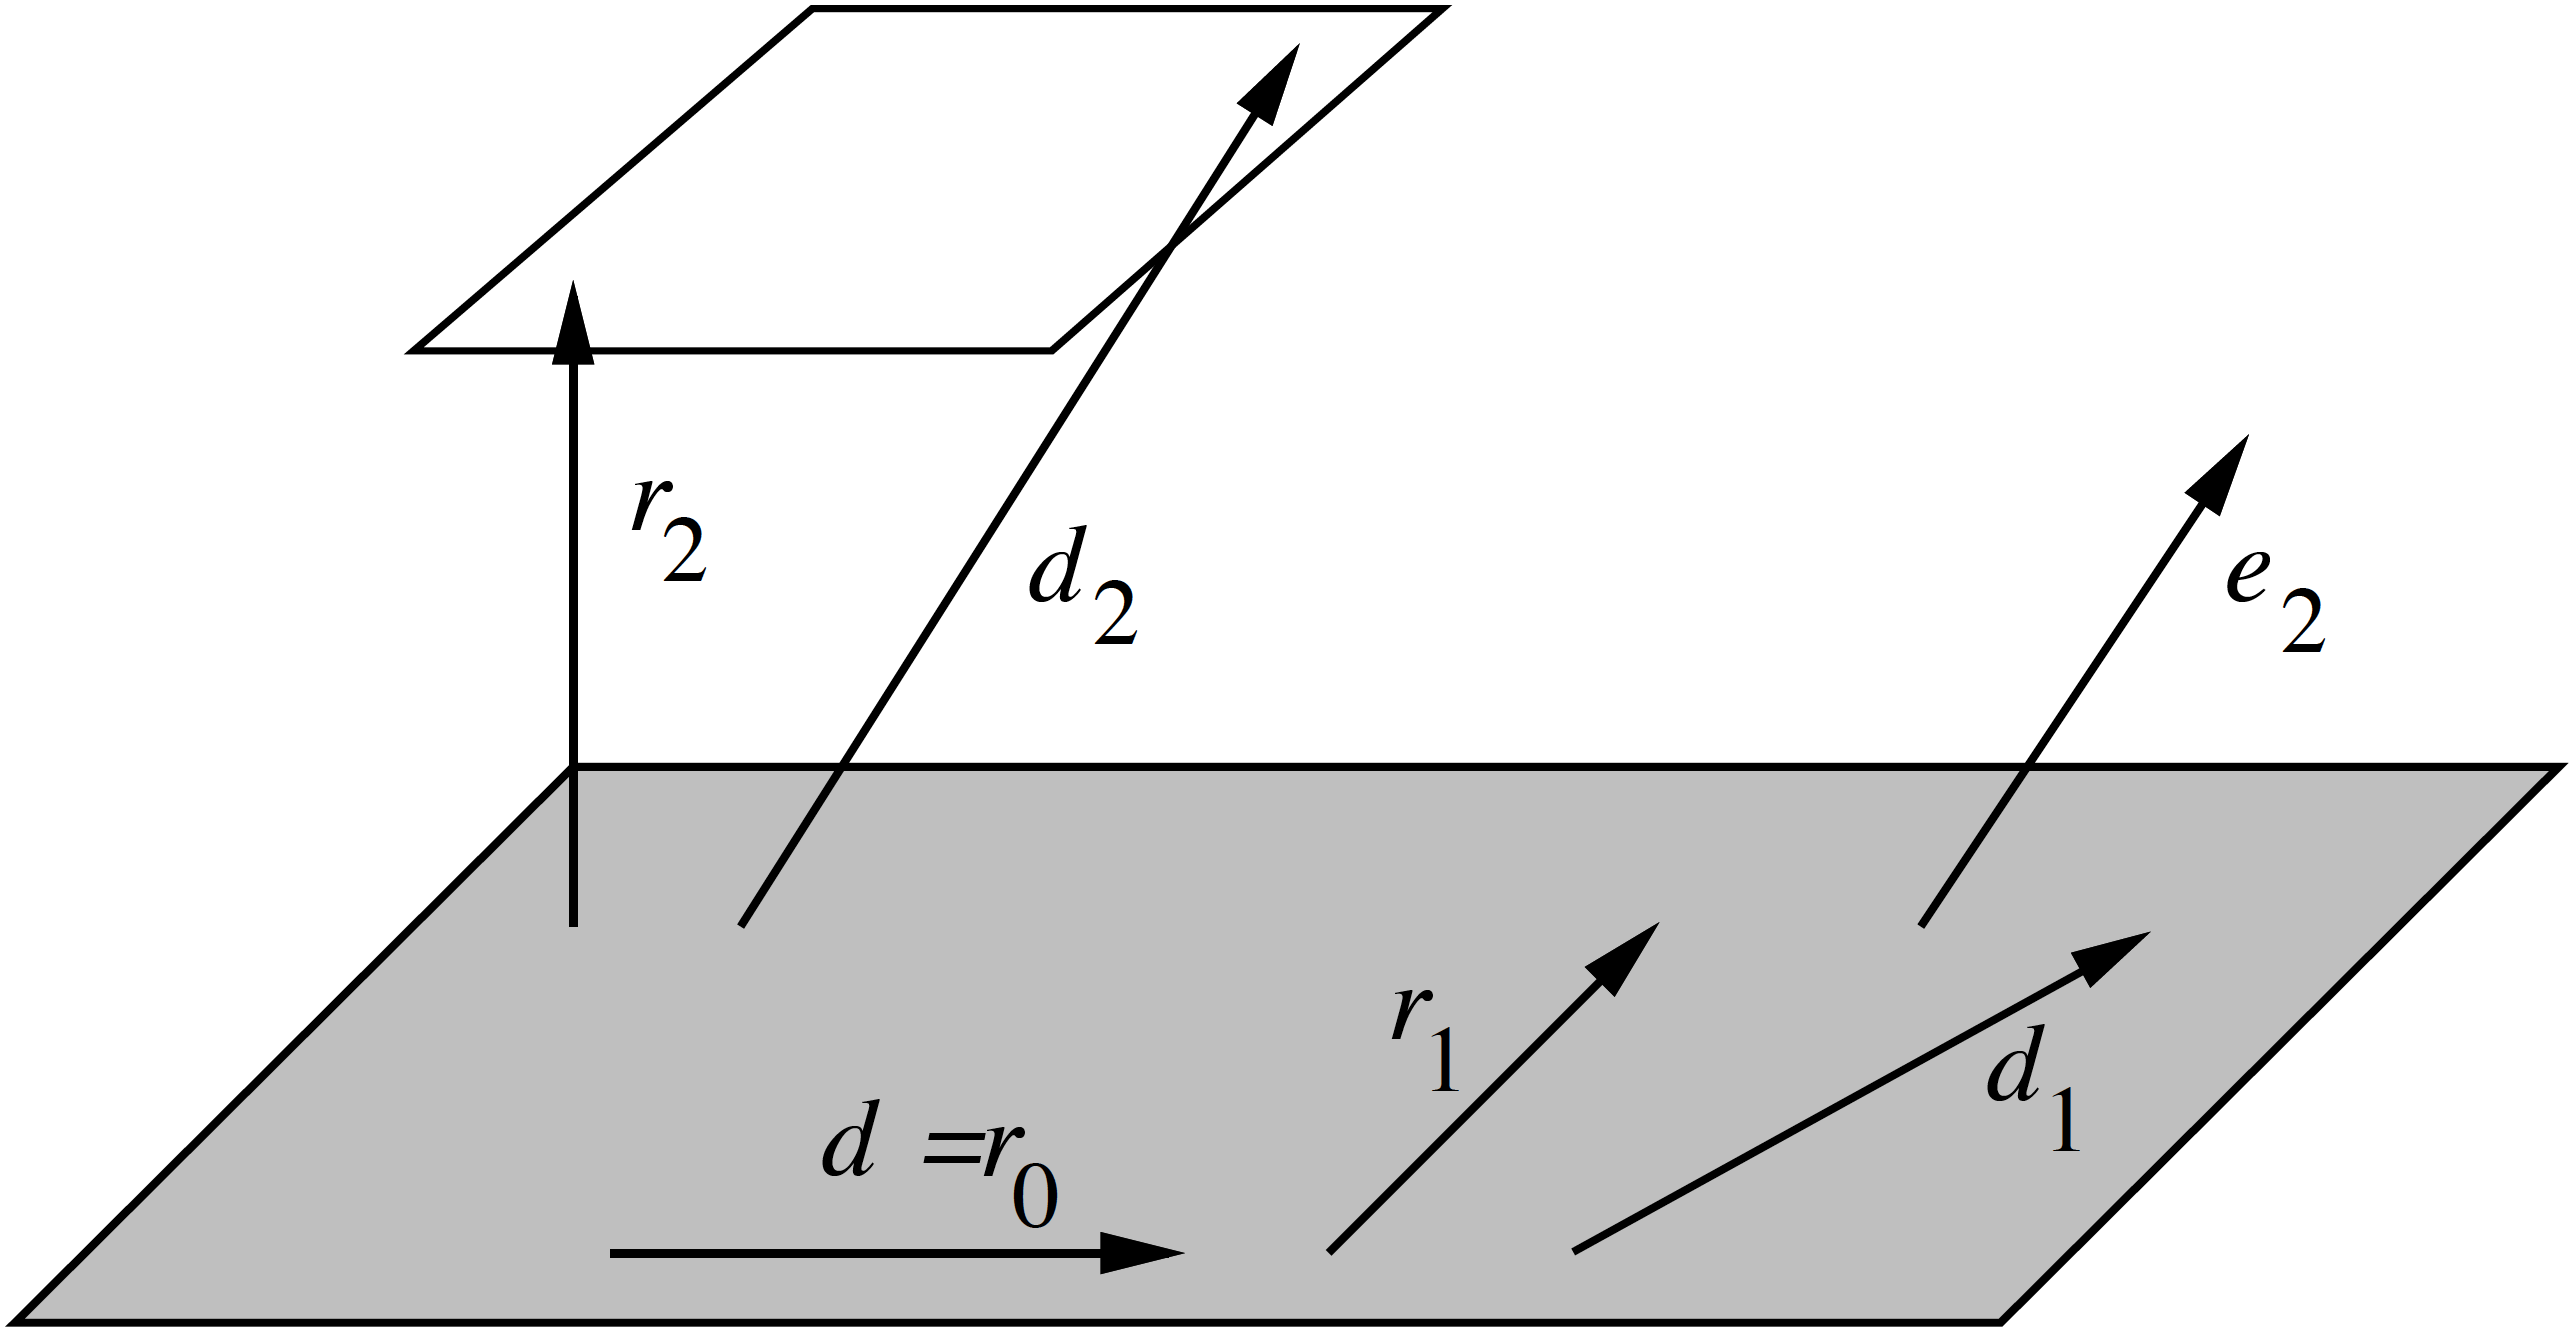
\includegraphics[width=.75\linewidth]{cg_ort.png}
    \caption{Il piano scuro è il sottospazio $\mathcal{K}_2$. Notiamo che $\mathbf{r_2}$ e $\mathbf{d}_2$ puntano su un piano parallelo a $\mathcal{K}_2$ (come conseguenza dell'ortogonalizzazione)}
    \label{fig:ortogonalizzazione}
\end{figure}
\begin{itemize}
\item Dalla Figura~\ref{fig:ortogonalizzazione} $\mathbf{d}_k^T\mathbf{r}_k=\mathbf{r}_k^T\mathbf{r}_k$, riscriviamo il passo di discesa come
$$
\alpha_k=\frac{\mathbf{r}_k^T \mathbf{r}_k}{\mathbf{d}_k^T A \mathbf{d}_k}
$$

\end{itemize}
\end{frame}


\begin{frame}
\frametitle{Velocità di convergenza}
\begin{itemize}
    \item Il metodo del gradiente coniugato converge al massimo in $\mathrm{n}$ iterazioni (in aritmetica esatta), e si ottiene che $$\|\mathbf{e}_{(k)}\|_A\leq\frac{2c^k}{1+c^{2k}}\|\mathbf{e}_{(0)}\|_A$$
    $$\|\mathbf{e}_{(k)}\|_A\leq2c^k\|\mathbf{e}_{(0)}\|_A$$
    $$ c=\frac{\sqrt{K(A)}-1}{\sqrt{K(A)}+1}.$$
    $$K(A)\text{ è il numero di condizionamento in norma 2 di } A$$
    
    \item Come metodo iterativo, viene arrestato quando il residuo relativo $E_{(k)}=\frac{\|\mathbf{r}_{(k)}\|}{\|\mathbf{r}_{(0)}\|}$ è minore di una tolleranza data. 
\end{itemize}
\end{frame}


%\begin{frame}
%\frametitle{Metodo del Gradiente Coniugato come Metodo di Krylov}
%\begin{itemize}
    %\item Il metodo del Gradiente Coniugato può essere visto come un particolare metodo di Krylov: la soluzione $\mathbf{x}^{\ast}$ appartiene al sottospazio di Krylov $\mathcal{K}_\mathrm{n}(A,\mathbf{r}_{(0)})$, e ad ogni iterazione anumenta di dimensione. 
    %\item Le condizioni di ortogonalita del vettore residuo rispetto alle n direzioni di discesa sono espresse nel sottospazio  $\mathcal{L}_\mathrm{n}\subseteq \mathbb{R}^n$, generato da queste ultime (che sono poste indipendenti tra loro): $$\mathcal{L}_\mathrm{n}=span\{ \mathbf{d}_{(0)},\dots,\mathbf{d}_{(n-1)} \} $$.
    
%\end{itemize}
%\end{frame}



\begin{frame}
\frametitle{Precondizionamento (I)}
\begin{itemize}
    \item La velocità di convergenza dipende quindi dal numero di condizionamento $\mathit{K(A)}$. %più è grande ka piu lenta conv.
    
    \item Per accelerare la convergenza dobbiamo diminuire il numero di condizionamento ($K(P^{-1}A)\ll K(A)$)
    \item Possiamo risolvere il \alert{sistema precondizionato} (equivalente a quello dato, $A\mathbf{x}=\mathbf{b}$)
    $$
    M^{-1}A\mathbf{x}=M^{-1}\mathbf{b}
    $$
    \item In generale se $M$ e $A$ sono simmetriche e definite non è detto che lo sia $M^{-1}A$, ma per ogni $M$ simmetrica, definita positiva esiste almeno una matrice $P$ tale che $PP^T=M$.
    \item Dato che $M^{-1}A$ e $P^{-1}AP^T$ hanno gli stessi autovalori possiamo scrivere il sistema equivalente
    $$
    P^{-1}AP^{-T}\mathbf{\hat{x}}=P^{-1}\mathbf{b},\, \mathbf{\hat{x}}=P^T\mathbf{x}
    $$
    
    \item $P^{-1}AP^{-T}$ è simmetrica e definita positiva.
    
\end{itemize}    
\end{frame}


\begin{frame}
\frametitle{Precondizionamento (II)}
\begin{itemize}
    \item Per tornare al caso del primo sistema precondizionato sfruttiamo l'equazione $M^{-1}=P^{-T}P^{-1}$
    \item Scegliendo $M$ stiammo operando un \textit{trade-off} tra la diminuzione del numero di condizionamento e il costo computazionale della risoluzione del sistema $\mathbf{s_{(k)}}=M^{-1}\mathbf{r_{(k)}}$ per trovare il residuo precondizionato $\mathbf{s_{(k)}}$.
   
    \item Esempio di algoritmi applicabili per calcolare $M$ sono:
    \begin{itemize}
    \item Precondizionamento di Jacobi
    \item Precondizionamento incompleto di Cholesky
    \end{itemize}    
   
    \item  La convergenza del metodo precondizionato è più veloce, poichè $K(A)$ è stato sostituito con $K(P^{-1}A)$: 
    $$\|\mathbf{e}_{(k)}\|_A\leq\frac{2c^k}{1+c^{2k}}\|\mathbf{e}_{(0)}\|_A,  c=\frac{\sqrt{K(P^{-1}A)}-1}{\sqrt{K(P^{-1}A)}+1}.$$
\end{itemize}    
\end{frame}

\begin{frame}
\frametitle{Metodo del gradiente coniugato (senza precondizionamento)}
\begin{itemize}
\item $\mathbf{d}_0=\mathbf{r}_0=\mathbf{b}-A\mathbf{x}_0$
\item $\alpha_k=\frac{\mathbf{r}_k^T \mathbf{r}_k}{\mathbf{d}_k^T A \mathbf{d}_k}$
\item $\mathbf{x}_{k+1}=\mathbf{x}_k+\alpha_k\mathbf{d}_{k}$
\item $\mathbf{r}_{k+1}=\mathbf{r}_k-\alpha_kA\mathbf{d}_{k}$
\item $\beta_{k+1}=\frac{\mathbf{r}_{k+1}^T\mathbf{r}_{k+1}}{\mathbf{r}_{k}^T\mathbf{r}_{k}}$
\item $\mathbf{d}_{k+1}=\mathbf{r}_{k+1}+\beta_{k+1}\mathbf{d}_k$
\end{itemize}    
\end{frame}

\begin{frame}\frametitle{Implementazione Matlab (senza precondizionamento)}

Dati come input
una matrice \lstinline[language=Matlab]{A}, 
il vettore dei termini noti \lstinline[language=Matlab]{b},
una guess iniziale \lstinline[language=Matlab]{x},
un numero massimo di iterazioni \lstinline[language=Matlab]{kmax}
e una tolleranza \lstinline[language=Matlab]{e}
\lstinputlisting[language=Matlab]{gradienteconiugato.m}
\end{frame}

\begin{frame}
\frametitle{Metodo del gradiente coniugato (con precondizionamento)}
\begin{itemize}
\item $\mathbf{r}_0=\mathbf{b}-A\mathbf{x}_0$
\item $\mathbf{d}_0=M^{-1}\mathbf{r}_0$
\item $\alpha_k=\frac{\mathbf{r}_k^TM^{-1} \mathbf{r}_k}{\mathbf{d}_k^T A \mathbf{d}_k}$
\item $\mathbf{x}_{k+1}=\mathbf{x}_k+\alpha_k\mathbf{d}_{k}$
\item $\mathbf{r}_{k+1}=\mathbf{r}_k-\alpha_kA\mathbf{d}_{k}$
\item $\beta_{k+1}=\frac{\mathbf{r}_{k+1}^TM^{-1}\mathbf{r}_{k+1}}{\mathbf{r}_{k}^TM^{-1}\mathbf{r}_{k}}$
\item $\mathbf{d}_{k+1}=M^{-1}\mathbf{r}_{k+1}+\beta_{k+1}\mathbf{d}_k$
\end{itemize}    
\end{frame}

\begin{frame}\frametitle{Implementazione Matlab (con precondizionamento)}
Dati come input
una matrice \lstinline[language=Matlab]{A}, 
il vettore dei termini noti \lstinline[language=Matlab]{b},
una guess iniziale \lstinline[language=Matlab]{x},
la matrice di precondizionamento \lstinline[language=Matlab]{M},
un numero massimo di iterazioni \lstinline[language=Matlab]{kmax}
e una tolleranza \lstinline[language=Matlab]{e}
\lstinputlisting[language=Matlab]{gradienteconiugatoprecondizionato.m}
\end{frame}

\begin{frame}
\frametitle{Considerazioni finali}
    Svantaggi
    \begin{itemize}
        \item In quanto metodi iterativi, sono soggetti a errori di troncamento. %ci si ferma ad un certo k
    \end{itemize}
    Vantaggi
    \begin{itemize}
        \item Possibilità di implementare questi metodi in versione \textit{matrix-free}, ovvero ad ogni iterazione basta solo calcolare un prodotto matrice-vettore, e altre operazioni meno computazionalmente costose. %quindi possiamo allocare meno memoria, e questo è buono quando ci sono problemi di grandi dimensioni, ed è utile x parallelismo su più cpu.
        \item Se la matrice è \alert{sparsa}, è possibile memorizzare i suoi elementi a un costo limitato ($O(n)$ invece di $O(n^2)$). Non è detto però i suoi fattori siano matrici sparse, quindi non è consigliabile applicare metodi di fattorizzazione.
        
    \end{itemize}
    %Confronto
    %\begin{itemize}
        %\item Convergenza del metodo del gradiente coniugato in meno iterazioni rispetto alla dimensione n della matrice A (calcolando invece la soluzione attraverso Cramer o con i metodi diretti ci sono operazioni matrice-matrice che possono risultare molto dispendiose).
        %\end{itemize}
\end{frame}

\begin{frame}{Confronto Gradiente - Gradiente Coniugato}
    \begin{figure}
    \centering
    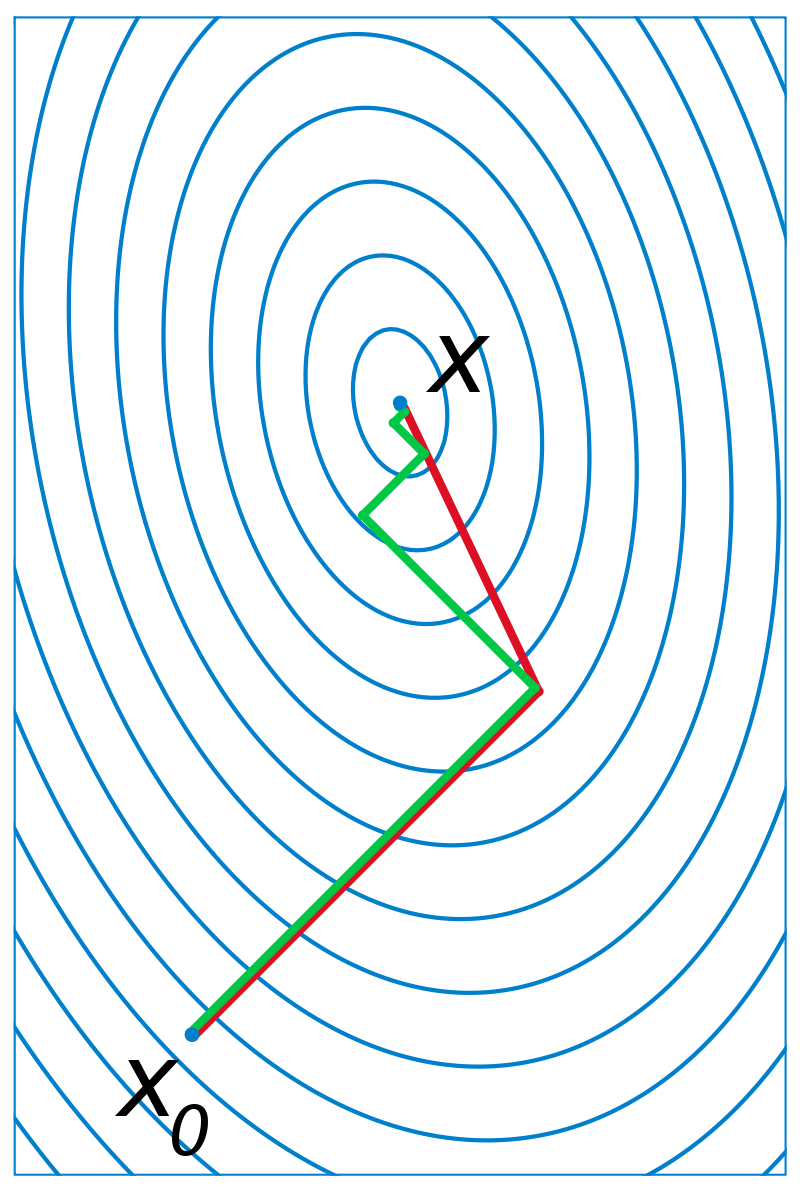
\includegraphics[width=.35\linewidth]{cg_comp.png}
    \caption{Confronto tra il numero di iterazioni dei due metodi )in verde il gradiente e in rosso il gradiente coniugato)}
Come si può osservare dalla figura, il metodo del Gradiente esegue molte più iterazioni rispetto al  metodo del Gradiente Coniugato. 
\end{figure}
\end{frame}

\section{GMRES}\label{sec:sec3}


\begin{frame} 
\begin{center}
\begin{tabular}{ c }
\hline\\
\textbf{Generalized Minimal RESidual} \\ [0.5ex]
risoluzione di un sistema lineare tramite sottospazio di Krylov\\ \\
 \hline
\end{tabular}
\end{center}
\end{frame}


\begin{frame} \frametitle{GMRES}
\begin{itemize}
    \item \textbf{GMRES} (Generalized Minimal RESidual) è uno dei metodi di Krylov utilizzato per risolvere il sistema lineare $Ax = b$ tramite il sottospazio
    $\mathcal{K}_\mathrm{n}$ in modo tale da rendere minima la norma Euclidea del residuo: $$\|\mathbf{b}-A\mathbf{x_n}\|_2.$$
    \item Sia $K_n$ la matrice $m x n$ di Krylov, composta da spazi colonne A$\mathcal{K}_\mathrm{n}$. Inanzitutto si moltiplica $K_n$ per A, per cui il problema diventa trovare un vettore $\mathbf{c}\in\mathbb{C}^n$, tale per cui il residuo $\|AK_n\mathbf{c}-\mathbf{b}\|_2$ sia minimo. 
    \item Questa formula è risolvibile con fattorizzazione QR, ma $AK_n$ diventa \textbf{numericamente instabile} al crescere di $n$, quindi si utilizza \alert{l'iterazione di Arnoldi} per costruire una base di vettori ortonormali.
\end{itemize}
\end{frame}


\begin{frame} \frametitle{L'iterazione di Arnoldi (I)}
\begin{itemize}
    \item Si definisce $Q_n$ come la matrice, i cui vettori formano una base ortonormale di $\mathcal{K}_\mathrm{n}$. Il problema consiste ora nella ricerca di $\mathbf{y}\in\mathbb{C}^n$ tale per cui: $$\|AQ_n\mathbf{y}-\mathbf{b}\|_2 = minimo,$$ riducendo così le dimensioni del problema da $m x n$ a $(n+1) x n$.
    \item L'iterazione di Arnoldi dimostra che $AQ_n = Q_{n+1}\mathcal{H}_n$ (con $\mathcal{H}_n$ la matrice alta-sinistra, $(n+1) x n$, della matrice di Hessenberg). Il problema quindi diventa:$$\|Q_{n+1}\mathcal{H}_n\mathbf{y}-\mathbf{b}\|_2 = minimo.$$ 
\end{itemize}
\end{frame}


\begin{frame} \frametitle{L'iterazione di Arnoldi (II)}
\begin{itemize}
    \item Moltiplicando entrambi i membri per $Q^*_{n+1}$ si ottiene: $$\|\mathcal{H}_n\mathbf{y}-Q^*_{n+1}\mathbf{b}\|_2 = minimo.$$
    \item Si osserva che $Q^*_{n+1}\mathbf{b}=\|\mathbf{b}\|\mathbf{e_1}$, con $\mathbf{e_1}=(1,0,0,\dots)^*$, quindi il problema 
    finale è:$$\|\mathcal{H}_n\mathbf{y}-\|\mathbf{b}\|\mathbf{e_1}\|_2 = minimo.$$ Questa equazione è risolvibile con l'approssimazione ai minimi quadrati.
\end{itemize}
\end{frame}


\begin{frame} 
\begin{center}
\begin{tabular}{ c }
\hline\\
\textbf{Generalized Minimal RESidual} \\ [0.5ex]
applicazione nel calcolo polinomiale\\ \\
 \hline
\end{tabular}
\end{center}
\end{frame}


\begin{frame} 
\frametitle{GMRES Polinomi}
\begin{itemize}
    \item Il metodo GMRES è utilizzabile anche nel calcolo polinomiale.
    \item Dato $p_n\in P_n$, con $p_n(0)=1$ si definisce $x_n=q_n(A)\mathbf{b}$ e $r_n=p_n(A)\mathbf{b}$. Il problema consiste nel calcolare $p_n\in P_n$ tale che $$\|r_n\|=minimo.$$
\end{itemize}
\end{frame}


\begin{frame} \frametitle{Velocità di convergenza}\framesubtitle{Quanto deve valere \textbf{n} (numero di iterazioni) per soddisfare la tolleranza?}
    $$ \frac{\|r_n\|}{\|\mathbf{b}\|}  < tolleranza$$
\begin{itemize}
    \item Osservazione 1: convergenza monotona $\|r_{n+1}\|\leq \|r_n\|$.
    \item Osservazione 2: per $n\to \infty$, $\|r_{\infty} \|= 0$, a meno di errori di arrotondamento.
    \item Essendo $\|r_n\| = \|p_n(A) \mathbf{b}\| \leq\|p_n(A)\|\|\mathbf{b}\|$ risulta che solo $p_n(A)$ influenza la velocità di convergenza: $$\frac{\|r_n\|}{\|\mathbf{b}\|} \leq inf\|p_n(A)\|,$$ con $p_n \in P_n$.
\end{itemize}
\end{frame}


\begin{frame} 
\begin{center}
\begin{tabular}{ c }
\hline\\
 \textbf{Analisi stazionaria efficiente} \\ [0.5ex]
  \textbf{basata sul metodo matrix-free nei sottospazi di Krylov}\\ \\
 \hline
\end{tabular}
\end{center}
\end{frame}


\begin{frame}
\frametitle{Matrix Free GMRES}\framesubtitle{Esempio applicativo del metodo: \textbf{circuiti analogici}}
\begin{itemize}
\item Più circuiti $\to$ più problemi per risolverli
\item Risposta del circuito dipende dagli ingressi (ampiezze, frequenze) $\to$ migliaia di punti da verificare
\item N equazioni $\to$ $N^3$ flops per Gauss, $N^2$ flops per metodi iterativi
\item Matrix-Free VS Iterativi: se N=400 $t_{It} \approx 10t_{MF}$
\end{itemize}
\end{frame}


\begin{frame}
\frametitle{Matrix Free GMRES}\framesubtitle{Algoritmo per calcolare la distorsione nei circuiti analogici}
%[CANCELLA](cerco stato stazionario periodico = le variabili di stato non dipendono dal tempo)[CANCELLA]
\begin{itemize}
\item I dati si ricavano simulando il circuito e misurando i valori ottenuti in un periodo T.
\begin{equation}
f(\mathbf{v}(t),t) = \mathbf{i}(\mathbf{v}(t)) + \mathbf{q}'(\mathbf{v}(t)) + \mathbf{u}(t) = 0	           
\end{equation}
\footnotetext{$\mathbf{v}$, $\mathbf{i}$, $\mathbf{q}$, $\mathbf{u} \in   \mathbb{R}^N$\\} 
\begin{equation}
\mathbf{v}(T) - \mathbf{v}(0) = 0 
\end{equation}
\item Dalla (1) e (2) si ricava  \begin{equation}
\mathbf{\phi}(\mathbf{v}(0),0,T) - \mathbf{v(0)}
 = 0
 \end{equation}
\item Dove \[ \phi = \int\limits_0^T f(\mathbf{v}(t),t) dt\]
%[CANCELLA](funzione di stato)[CANCELLA] 
\end{itemize}
\end{frame}


\begin{frame}
\frametitle{Matrix Free GMRES}
\framesubtitle{Iterazione di Newton (I)}
\begin{itemize}
\item Tramite il metodo di Newton alla (3) si ottiene l'iterazione\begin{equation}
\mathbf{v}_0^j = \mathbf{v}_0^{j-1} - [J_{\phi}(\mathbf{v}_0^{j-1},0,T) - I]^{-1}[\phi(\mathbf{v}_0^{j-1},0,T) - \mathbf{v}_0^{j-1}]
\end{equation}con $\mathbf{v}_0 = \mathbf{v}(t=0)$.       
\item Utilizzando opportuni passaggi(vedi dac95 paragrafo 2) si ricava la formula
\end{itemize} 
 \begin{equation}
\bigg[\frac{\mathbf{C}(\mathbf{v}_m^{l-1})}{h_m} + \mathbf{G}(\mathbf{v}_m^{l-1})\bigg](\mathbf{v}_m^l-\mathbf{v}_m^{l-1}) = - \frac{1}{h_m}(\mathbf{q}(\mathbf{v}_m^{l-1}) - \mathbf{q}(\mathbf{v}_{m-1})) - \mathbf{i}(\mathbf{v}_m^{l-1}) - \mathbf{u}_m
\tag{8}
\end{equation}
\end{frame}


\begin{frame}
\frametitle{Matrix Free GMRES}
\framesubtitle{Iterazione di Newton (II)}
Siano\\
\begin{itemize}
\item m = instante temporale%[CANCELLA](suddivido T in M instanti)[CANCELLA]
\item $h_m = t_m - t_{m-1}$
\item $\mathbf{C} = \frac{d\mathbf{q}}{d\mathbf{v}}$
\item $\mathbf{G} = \frac{d\mathbf{i}}{d\mathbf{v}}$ 
\item $J_f = \frac{\mathbf{C}(\mathbf{v}_m^{l-1})}{h_m} + \mathbf{G}(\mathbf{v}_m^{l-1})$
\end{itemize}
 La sensibilità si esprime come
 \begin{equation}
J_f(\mathbf{v}_m)\frac{d\mathbf{v}_m}{d\mathbf{v}_0} = \frac{\mathbf{C}(\mathbf{v}_{m-1})}{h_m}\frac{d\mathbf{v}_{m-1}}{d\mathbf{v}_0}
\tag{11}
\end{equation}
L'iterazione di Newton richiede circa $N^2$ flops.\footnote{N = dim($\mathbf{v}$)\\}
\end{frame}


\begin{frame}
\frametitle{Matrix Free GMRES}\framesubtitle{\textbf{Algoritmo (I)}. Per risolvere Ax = b con GMRES}
$\mathbf{x}_0 =$ Guess iniziale\\
$p_0 = b - A\mathbf{x}_0$ (direzione)\\
k = 1\\
do \{\\
$p^k = Ap^{k-1}$ (nuova direzione)\\
$p^k = p^k -\sum\limits_{j=0}^{k-1}\beta_{k,j}p^j$ (ortogonalizza)\\
cerca $\alpha_k$ in $x^k = x^{k -1} + \alpha_kp^k$ tale che\\
$\|r^k\| = \|\mathbf{b} - A\mathbf{x}^k\|$ minimo\\
$k = k + 1$\\
\} while($\|r^k\| < tolerance_{GMRES}$)\\
$\mathbf{x}^k = soluzione$
\end{frame}


\begin{frame}
\frametitle{Matrix Free GMRES}
\begin{itemize}
\item Il costo elevato dell'iterazione di Newton è causato dal calcolo di $ A = J_\phi - I$: $dim(A) = N^2$
\item Il GMRES matrix free consente di risolvere il sistema senza memorizzare l'intera matrice A  
%[CANCELLA(il computer memorizza A in forma sparsa,ovvero tiene in memoria solo i valori di A utili al calcolo della soluzione)CANCELLA]
\item 
Così facendo il calcolo di $J_\phi p^{k-1}$ richiede circa N operazioni\footnote{$J_\phi p^{k-1}$ serve a calcolare $Ap^{k-1}$ in ogni step k dell'iterazione \\}
\end{itemize}
\end{frame}


\begin{frame}
\frametitle{Matrix Free GMRES}
\begin{itemize}
\item $Ap^{k-1} = (J_\phi - I)p^{k-1}$ è approssimabile a meno di un errore $\epsilon$ \\\begin{equation} \frac{\phi(\mathbf{v}_0 + \epsilon p^{k-1},0,T) - \phi (\mathbf{v}_0)}{\epsilon} - p^{k-1}
\tag{12}
\end{equation}
%\item [CANCELLA](vedi frase dac 95 sotto la(12))[CANCELLA]
\item L'algoritmo utilizzato per risolvere la (12) richiede lo stesso numero di operazioni necessario a calcolare una sola colonna di $J_\phi$ con il metodo di Newton
\item Salvare $\mathbf{C}(\mathbf{v}_m)$ e fattorizzare LU $J_f(\mathbf{v}_m)$ ad ogni passo per applicare:
\end{itemize}
\begin{equation}
J_f(\mathbf{v}_m)\frac{d\mathbf{v}_m}{d\mathbf{v}_0} = \frac{\mathbf{C}(\mathbf{v}_{m-1})}{h_m}\frac{d\mathbf{v}_{m-1}}{d\mathbf{v}_0}
\tag{11}
\end{equation}  
\end{frame}


\begin{frame}
\frametitle{Matrix Free GMRES}\framesubtitle{\textbf{Algoritmo (II)}. Per risolvere Ax = b matrix free}
$\mathbf{v}_0 =$ Guess iniziale \\
 For j = 1 to Max Newton \{ \\
 $\int\limits_{0}^{T} (1) dt$ con $\mathbf{v}_0 = \mathbf{v}_0^{j-1}$ \\
 For m = 1 to M \{ \\
 Risolvi la (6) \\
 Salva $J_f(\mathbf{v}_m)$ e $\mathbf{C}(\mathbf{v}_m)$ \\
 \}\\
 Risolvi $(J_\phi(\mathbf{v}^{j-1}) - I)\delta\mathbf{v}^j = \mathbf{v}^{j-1} - \phi(\mathbf{v}^{j-1})$ con GMRES\\
 Nel GMRES calcola $p^{k+1} = J_\phi(\mathbf{v}^{j-1})p^k$ usando\\
 $p^{k+1} = p^k$ \\
 For m = 1 to M risolvi $J_f(\mathbf{v}_m)p^{k+1} = \mathbf{C}(\mathbf{v}_{m-1})p^{k+1}$ \\
 $\mathbf{v}^j = \mathbf{v}^{j-1} + \delta\mathbf{v}^j$ \\
 se $\|\delta\mathbf{v}^j\| < tolleranza_{Newton}$ return\\
 \}
\end{frame}


\begin{frame} \frametitle{Matrix Free GMRES}
\begin{figure}
    \centering
    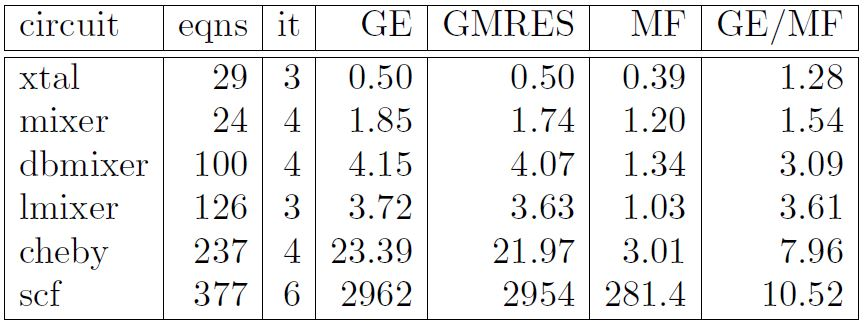
\includegraphics[width=.75\linewidth]{Tabella1.JPG}
    \caption{Comparazione\footnotemark di metodi diversi per la risoluzione dei circuiti elettronici.}
%    \label{fig:my_label}
\end{figure}
%Se la figura ha un'etichetta la si può usare per fare riferimento
%alla figura nel testo : Figura~\ref{fig:my_label}
\footnotetext{Risultati ottenuti con HP712/80 workstation.}
\end{frame}


\begin{frame} \frametitle{Matrix Free GMRES}
\begin{figure}
    \centering
    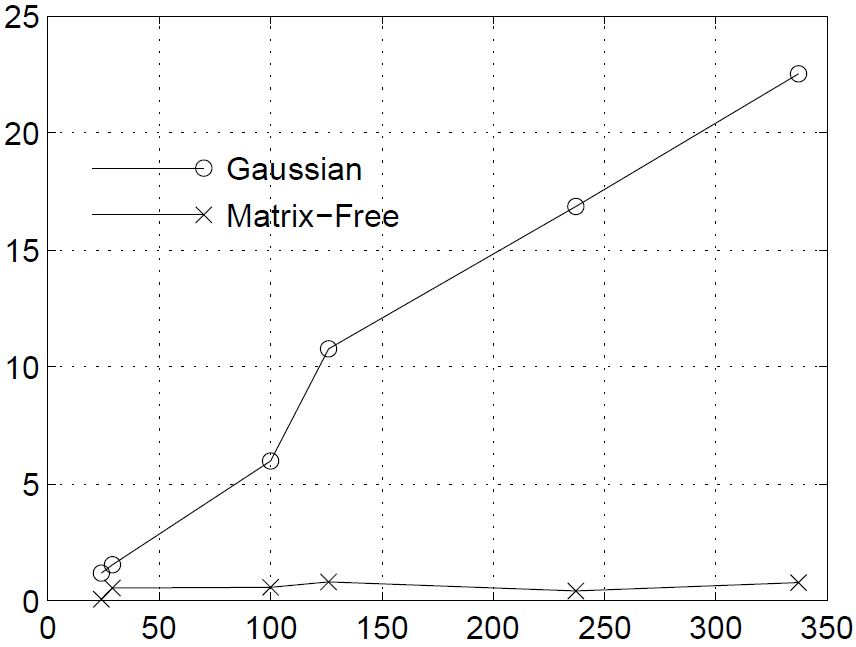
\includegraphics[width=.75\linewidth]{Figura1.JPG}
    \caption{Rapporto tra lo "shooting update time" e il costo di elaborazione del calcolo di una singola operazione.}
\end{figure}

\end{frame}


\begin{frame} \frametitle{Matrix Free GMRES}
\begin{figure}
    \centering
    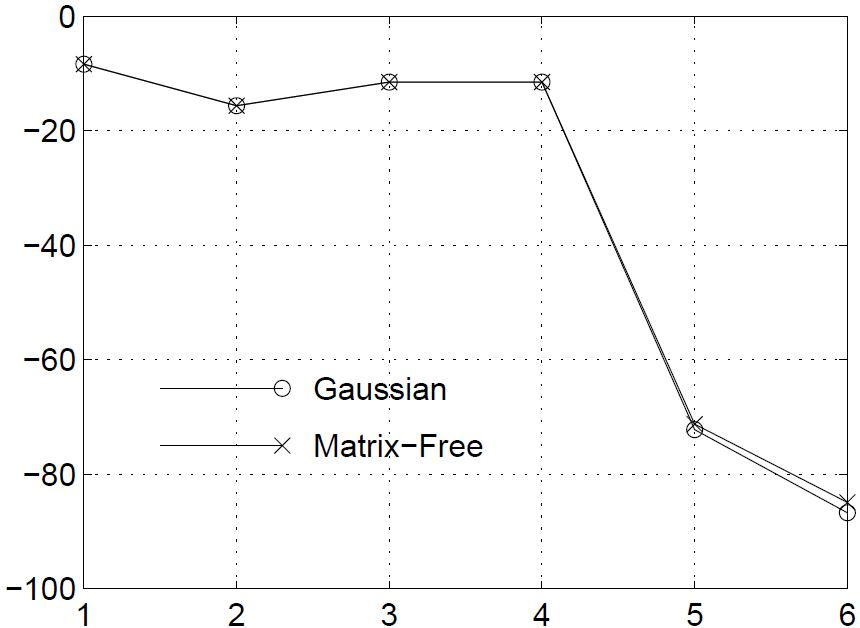
\includegraphics[width=.75\linewidth]{Figura2.JPG}
    \caption{Il grado di convergenza del metodo di Newton comparato al metodo Matrix Free.}
\end{figure}
\end{frame}
\end{document}